% Options for packages loaded elsewhere
\PassOptionsToPackage{unicode}{hyperref}
\PassOptionsToPackage{hyphens}{url}
%
\documentclass[
]{article}
\usepackage{amsmath,amssymb}
\usepackage{lmodern}
\usepackage{iftex}
\ifPDFTeX
  \usepackage[T1]{fontenc}
  \usepackage[utf8]{inputenc}
  \usepackage{textcomp} % provide euro and other symbols
\else % if luatex or xetex
  \usepackage{unicode-math}
  \defaultfontfeatures{Scale=MatchLowercase}
  \defaultfontfeatures[\rmfamily]{Ligatures=TeX,Scale=1}
\fi
% Use upquote if available, for straight quotes in verbatim environments
\IfFileExists{upquote.sty}{\usepackage{upquote}}{}
\IfFileExists{microtype.sty}{% use microtype if available
  \usepackage[]{microtype}
  \UseMicrotypeSet[protrusion]{basicmath} % disable protrusion for tt fonts
}{}
\makeatletter
\@ifundefined{KOMAClassName}{% if non-KOMA class
  \IfFileExists{parskip.sty}{%
    \usepackage{parskip}
  }{% else
    \setlength{\parindent}{0pt}
    \setlength{\parskip}{6pt plus 2pt minus 1pt}}
}{% if KOMA class
  \KOMAoptions{parskip=half}}
\makeatother
\usepackage{xcolor}
\usepackage[margin=0.75in]{geometry}
\usepackage{graphicx}
\makeatletter
\def\maxwidth{\ifdim\Gin@nat@width>\linewidth\linewidth\else\Gin@nat@width\fi}
\def\maxheight{\ifdim\Gin@nat@height>\textheight\textheight\else\Gin@nat@height\fi}
\makeatother
% Scale images if necessary, so that they will not overflow the page
% margins by default, and it is still possible to overwrite the defaults
% using explicit options in \includegraphics[width, height, ...]{}
\setkeys{Gin}{width=\maxwidth,height=\maxheight,keepaspectratio}
% Set default figure placement to htbp
\makeatletter
\def\fps@figure{htbp}
\makeatother
\setlength{\emergencystretch}{3em} % prevent overfull lines
\providecommand{\tightlist}{%
  \setlength{\itemsep}{0pt}\setlength{\parskip}{0pt}}
\setcounter{secnumdepth}{5}
\newlength{\cslhangindent}
\setlength{\cslhangindent}{1.5em}
\newlength{\csllabelwidth}
\setlength{\csllabelwidth}{3em}
\newlength{\cslentryspacingunit} % times entry-spacing
\setlength{\cslentryspacingunit}{\parskip}
\newenvironment{CSLReferences}[2] % #1 hanging-ident, #2 entry spacing
 {% don't indent paragraphs
  \setlength{\parindent}{0pt}
  % turn on hanging indent if param 1 is 1
  \ifodd #1
  \let\oldpar\par
  \def\par{\hangindent=\cslhangindent\oldpar}
  \fi
  % set entry spacing
  \setlength{\parskip}{#2\cslentryspacingunit}
 }%
 {}
\usepackage{calc}
\newcommand{\CSLBlock}[1]{#1\hfill\break}
\newcommand{\CSLLeftMargin}[1]{\parbox[t]{\csllabelwidth}{#1}}
\newcommand{\CSLRightInline}[1]{\parbox[t]{\linewidth - \csllabelwidth}{#1}\break}
\newcommand{\CSLIndent}[1]{\hspace{\cslhangindent}#1}
\usepackage{setspace}
\setcounter{section}{1}
\singlespacing
\usepackage{wrapfig}
\usepackage{lipsum}
\usepackage{float}
\usepackage{lineno}
\usepackage{amsmath}
\linenumbers
\renewcommand{\thefigure}{S\arabic{figure}}
\renewcommand{\thetable}{S\arabic{table}}
\renewcommand{\theequation}{S.\arabic{equation}}
\renewcommand{\thesection}{S\arabic{section}}
\usepackage{fancyhdr}
\setlength{\parskip}{\baselineskip}
\usepackage{tocloft}
\setlength{\cftbeforesecskip}{6pt}
\usepackage{booktabs}
\usepackage{makecell}
\DeclareMathOperator{\EX}{\mathbb{E}}% expected value
\usepackage{dcolumn}
\usepackage{booktabs}
\usepackage{longtable}
\usepackage{array}
\usepackage{multirow}
\usepackage{wrapfig}
\usepackage{float}
\usepackage{colortbl}
\usepackage{pdflscape}
\usepackage{tabu}
\usepackage{threeparttable}
\usepackage{threeparttablex}
\usepackage[normalem]{ulem}
\usepackage{makecell}
\usepackage{xcolor}
\ifLuaTeX
  \usepackage{selnolig}  % disable illegal ligatures
\fi
\IfFileExists{bookmark.sty}{\usepackage{bookmark}}{\usepackage{hyperref}}
\IfFileExists{xurl.sty}{\usepackage{xurl}}{} % add URL line breaks if available
\urlstyle{same} % disable monospaced font for URLs
\hypersetup{
  pdftitle={Supporting information for: Wilson et al. 2022. The role of spatial structure in at-risk metapopulation recoveries. In: Ecological Applications.},
  hidelinks,
  pdfcreator={LaTeX via pandoc}}

\title{Supporting information for: Wilson \emph{et al.} 2022. The role
of spatial structure in at-risk metapopulation recoveries. In:
\emph{Ecological Applications}.}
\usepackage{etoolbox}
\makeatletter
\providecommand{\subtitle}[1]{% add subtitle to \maketitle
  \apptocmd{\@title}{\par {\large #1 \par}}{}{}
}
\makeatother
\subtitle{\textbf{Appendix S1:} Overview of metapopulation model
description \& detailed results}
\author{Kyle L. Wilson\(^\textup{1,2}\)\footnote{Corresponding author -
  email:
  \href{mailto:klwilson.ccira@gmail.com}{\nolinkurl{klwilson.ccira@gmail.com}}},
Alexandra C. Sawyer\(^\textup{1}\), Anna Potapova\(^\textup{1}\), Colin
J. Bailey\(^\textup{1}\),Daniella LoScerbo\(^\textup{3,4}\),\\
Elissa K. Sweeney-Bergen\(^\textup{1,5}\), Emma E.
Hodgson\(^\textup{1,4}\), Kara J. Pitman\(^\textup{1}\), Karl M.
Seitz\(^\textup{1}\),\\
Lauren Law\(^\textup{1,6}\), Luke Warkentin\(^\textup{1,7}\), Samantha
M. Wilson\(^\textup{1}\), William I. Atlas\(^\textup{1,8}\),\\
Douglas C. Braun\(^\textup{3,5}\), Matthew R. Sloat\(^\textup{8}\), M.
Tim Tinker\(^\textup{9}\),\\
and Jonathan W. Moore\(^\textup{1,3}\)\\
\strut \\
\(^\textup{1}\)Earth to Ocean Research Group, Simon Fraser University\\
\(^\textup{2}\)Central Coast Indigenous Resource Alliance, Campbell
River, BC\\
\(^\textup{3}\)Resource and Environmental Management, Simon Fraser
University\\
\(^\textup{4}\)Fisheries \& Oceans Canada, Cultus Lake Laboratory,
Cultus Lake, BC\\
\(^\textup{5}\)Ministry of Forests, Lands, Natural Resource Operations,
and Rural Development, Smithers, BC\\
\(^\textup{6}\)Fisheries \& Oceans Canada, Salmonid Enhancement Program,
Nanaimo, BC\\
\(^\textup{7}\)Fisheries \& Oceans Canada, North Coast Stock Assessment,
Smithers, BC\\
\(^\textup{8}\)Wild Salmon Center, Portland, OR\\
\(^\textup{9}\)Ecology and Evolutionary Biology, University of
California Santa Cruz}
\date{14 December 2022}

\begin{document}
\maketitle

\centering
\raggedright
\renewcommand{\baselinestretch}{1}\normalsize
\tableofcontents
\renewcommand{\baselinestretch}{0.75}\normalsize
\newpage

\pagestyle{fancy}
\fancyhead[LO,LE]{Wilson \textit{et al.}}
\fancyhead[RO,RE]{\textbf{Appendix S1}: Spatial recoveries in metapopulations}

\hypertarget{metapopulation-model}{%
\subsection{Metapopulation model}\label{metapopulation-model}}

\hypertarget{local-metapopulation-dynamics}{%
\subsubsection{Local \& metapopulation
dynamics}\label{local-metapopulation-dynamics}}

Our metapopulation was defined by a set of \(P\) local populations for a
species with a one year generation time with time-dynamics that follows
birth (i.e., recruitment \emph{R}), immigration, death, and emigration
processes typical to metapopulation theory and tested the role of
multiple local and regional processes (Anderson et al. 2015; Fullerton
et al. 2016; Zelnik et al. 2019; Bowlby \& Gibson 2020; Okamoto et al.
2020):

\begin{align}
N_{i,t}= (1-d_{i,t})(R_{i,t}+{\sum\limits_{\substack{j=1 \\ j\neq i}}^{P} \omega p_{i,j}R_{j,t}}-\omega R_{i,t})
\end{align}

where \(N_{i,t}\) was the number of adults in patch \emph{i} at time
\emph{t}, \(R_{i,t}\) was the number of recruits at time \emph{t},
\({\sum\limits_{\substack{j=1 \\ j\neq i}}^{P} \omega p_{i,j}R_{j,t}}\)
was the number of recruits immigrating into patch \emph{i} from any
other patch, \(\omega\) was the proportion of local recruits to
disperse, \(p_{i,j}\) was a distance-dependent dispersal function, and
\(d_{i,t}\) was the proportion of post-dispersal recruits lost from the
disturbance regime.

Figure S1 shows how local patch recruitment at time \emph{t} depended on
adult densities at \emph{t-1} and followed a reparameterized
Beverton-Holt function based on compensation ratio (Box 3.1 in Walters
\& Martell 2004) and ignoring age-structure to model adult-to-adult
dynamics, i.e., setting \(\phi_{E_{0}}=1\), \(\phi_{B_{0}}=1\) and
\(R_0=N_0\) in Table 3 in Forrest et al. (2010):

\begin{align}
R_{i,t}=\cfrac{\alpha_iN_{i,t-1}}{1+\cfrac{\alpha_i-1}{\beta_i}N_{i,t-1}}\epsilon_{i,t}
\end{align}

where \(\alpha_i\) was the recruitment compensation ratio, \(\beta_i\)
was local patch carrying capacity, and \(\epsilon_{i,t}\) was
lognormally distributed deviates to introduce stochastic recruitment
dynamics.

Resource monitoring often occurs at the scale of the whole
metapopulation by sampling aggregate abundances from multiple local
populations to (Anderson et al. 2015; Moore et al. 2021), hence we
define metapopulation adults as:

\begin{align}
{A}_t = \sum_{i=1}^{P} N_{i,t}
\end{align}

with metapopulation recruits:

\begin{align}
K_t = \sum_{i=1}^{P} R_{i,t}
\end{align}

Monitoring at the scale of the whole metapopulation can produce
productivity relationships that aggregates the population dynamics and
productivity among all local populations. For example, take a two patch
metapopulation model (Figure S1) that each vary in demographic shape
parameters \(\alpha_1=2; \alpha_2=4\) and \(\beta_1=100; \beta_2=200\).
Here, recruitment compensation from local patches \(\alpha_i\) gets
averaged across the metapopulation leading to an average compensation
ratio \(\bar{\alpha}\) of 3. Likewise, the total carrying capacity of
the metapopulation \(\bar{\beta}\) becomes the summation of local patch
carrying capacities \(\sum\beta_i\), which was 300. This scale of
monitoring generates the following local patch and metapopulation
dynamics:

\begin{figure}[H]

{\centering 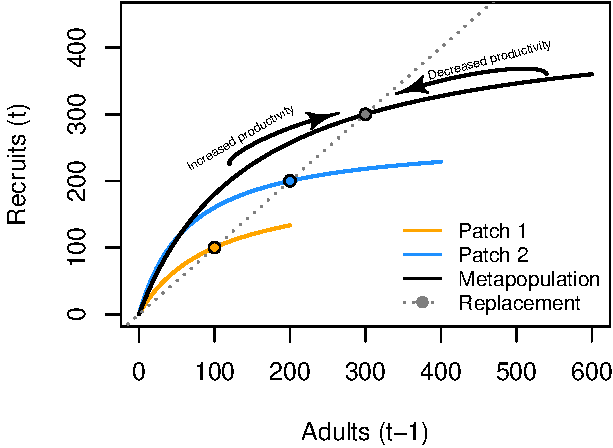
\includegraphics{Managing_for_ecological_surprises_in_metapopulations_files/figure-latex/recruit curves-1} 

}

\caption{Density dependence in metapopulation and local patch recruitment dynamics. Dashed line indicates the line of replacement, with equilbrium indicated by points. When populations fall below equilibrium points, per-capita productivity improves driving populations back towards equilibrium. When populations exceed their capacity, per-capita productivity decreases driving populations back towards equilibrium. At each point of the x-axis, the distance between the solid and dashed lines indicates the amount of recruitment above replacement, i.e., the surplus recruitment produced via compensatory density dependence.}\label{fig:recruit curves}
\end{figure}

\hypertarget{creating-the-spatial-networks}{%
\subsubsection{Creating the spatial
networks}\label{creating-the-spatial-networks}}

The next aspect to developing our metapopulation model was connecting
the set of patches to one another (Yeakel et al. 2014). We needed to
specify the number of patches, their arrangements (i.e., connections),
and how far apart they are from one another. We followed some classic
metapopulation and source-sink arrangements to create four networks that
generalize across a few real-world topologies: a linear habitat network
(e.g., coastline), a dendritic or branching network (e.g., coastal
rivers), a star network (e.g., mountain \& valley, or lake with inlet
tributaries), and a grid network (e.g., grasslands).

To make networks comparable, each spatial network type needs the same
leading parameters (e.g., number of patches \(P\) and mean distance
between neighboring patches \(\bar{d}\)). In this case, we set \(P\) to
\texttt{16} and \(\bar{d}\) to \texttt{1} unit (distance units are
arbitrary). We used the \texttt{igraph} package (Csardi \& Nepusz 2006)
to arrange our spatial networks as the following:

\begin{figure}[H]

{\centering 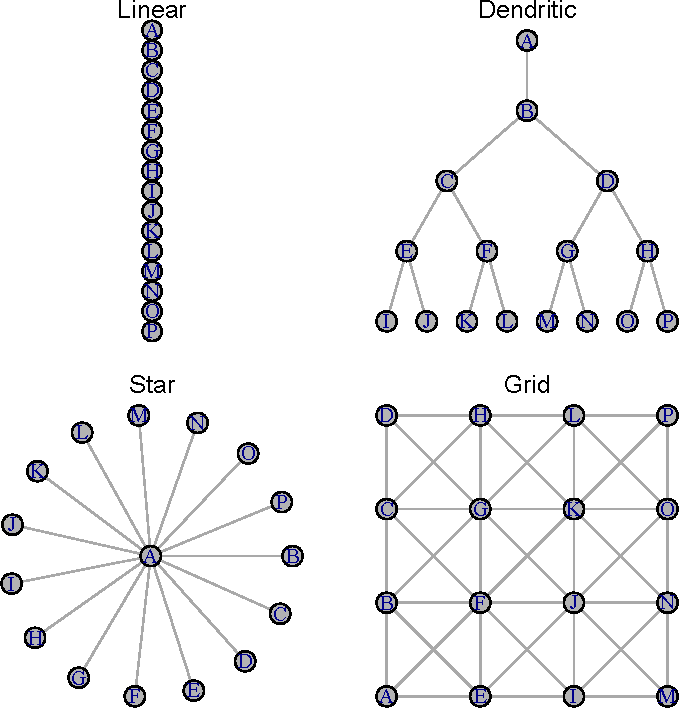
\includegraphics{Managing_for_ecological_surprises_in_metapopulations_files/figure-latex/networks-1} 

}

\caption{Four spatial network topologies.}\label{fig:networks}
\end{figure}

Note that distances between neighbor patches in the above networks are
equal. Table S1 shows an example dispersal matrix for a grid network.

\begin{table}

\caption{\label{tab:distance matrix}Example distance matrix between 16 patches within a grid network to affect distance-dependent dispersal rates.}
\centering
\begin{tabular}[t]{lrrrrrrrrrrrrrrrr}
\toprule
  & A & B & E & F & C & G & D & H & I & J & K & L & M & N & O & P\\
\midrule
A & 0 & 1 & 1 & 1 & 2 & 2 & 3 & 3 & 2 & 2 & 2 & 3 & 3 & 3 & 3 & 3\\
B & 1 & 0 & 1 & 1 & 1 & 1 & 2 & 2 & 2 & 2 & 2 & 2 & 3 & 3 & 3 & 3\\
E & 1 & 1 & 0 & 1 & 2 & 2 & 3 & 3 & 1 & 1 & 2 & 3 & 2 & 2 & 2 & 3\\
F & 1 & 1 & 1 & 0 & 1 & 1 & 2 & 2 & 1 & 1 & 1 & 2 & 2 & 2 & 2 & 2\\
C & 2 & 1 & 2 & 1 & 0 & 1 & 1 & 1 & 2 & 2 & 2 & 2 & 3 & 3 & 3 & 3\\
\addlinespace
G & 2 & 1 & 2 & 1 & 1 & 0 & 1 & 1 & 2 & 1 & 1 & 1 & 2 & 2 & 2 & 2\\
D & 3 & 2 & 3 & 2 & 1 & 1 & 0 & 1 & 3 & 2 & 2 & 2 & 3 & 3 & 3 & 3\\
H & 3 & 2 & 3 & 2 & 1 & 1 & 1 & 0 & 3 & 2 & 1 & 1 & 3 & 2 & 2 & 2\\
I & 2 & 2 & 1 & 1 & 2 & 2 & 3 & 3 & 0 & 1 & 2 & 3 & 1 & 1 & 2 & 3\\
J & 2 & 2 & 1 & 1 & 2 & 1 & 2 & 2 & 1 & 0 & 1 & 2 & 1 & 1 & 1 & 2\\
\addlinespace
K & 2 & 2 & 2 & 1 & 2 & 1 & 2 & 1 & 2 & 1 & 0 & 1 & 2 & 1 & 1 & 1\\
L & 3 & 2 & 3 & 2 & 2 & 1 & 2 & 1 & 3 & 2 & 1 & 0 & 3 & 2 & 1 & 1\\
M & 3 & 3 & 2 & 2 & 3 & 2 & 3 & 3 & 1 & 1 & 2 & 3 & 0 & 1 & 2 & 3\\
N & 3 & 3 & 2 & 2 & 3 & 2 & 3 & 2 & 1 & 1 & 1 & 2 & 1 & 0 & 1 & 2\\
O & 3 & 3 & 2 & 2 & 3 & 2 & 3 & 2 & 2 & 1 & 1 & 1 & 2 & 1 & 0 & 1\\
\addlinespace
P & 3 & 3 & 3 & 2 & 3 & 2 & 3 & 2 & 3 & 2 & 1 & 1 & 3 & 2 & 1 & 0\\
\bottomrule
\end{tabular}
\end{table}

\hypertarget{dispersal}{%
\subsubsection{Dispersal}\label{dispersal}}

Dispersal from patch \emph{i} into patch \emph{j} depends on constant
dispersal rate \(\omega\) (defined as the proportion of total local
recruits that will disperse) and an exponential distance-decay function
between \emph{i} and \emph{j} with distance cost to dispersal \(m\)
(Anderson et al. 2015; Fullerton et al. 2016):

\begin{align}
E_{i,j,t}=\omega R_{i,t}p_{i,j}
\end{align}

where \(E_{i,j}\) was the total dispersing animals from patch \emph{i}
into patch \emph{j} resulting from dispersal rate \(\omega\), total
number of local recruits \(R_{i,t}\), and probability of dispersal
between patches \(p_{i,j}\):

\begin{align}
p_{i,j}=\dfrac{e^{-md_{i,j}}}{\sum\limits_{\substack{j=1 \\ j\neq i}}^{P} e^{-md_{i,j}}}
\end{align}

where \(d_{i,j}\) was the pairwise distance between patches, \(m\) was
the distance cost to dispersal. The summation term in the denominator
normalizes the probability of moving to any patch to between 0 and 1
with the constraint that dispersers cannot move back into their home
patch (i.e., \(j\neq i\). With \(\bar{d}= 1\), \(m=0.5\),
\(\omega=0.1\), \(R_{i,t}=100\) in a linear network):

\begin{figure}[H]

{\centering 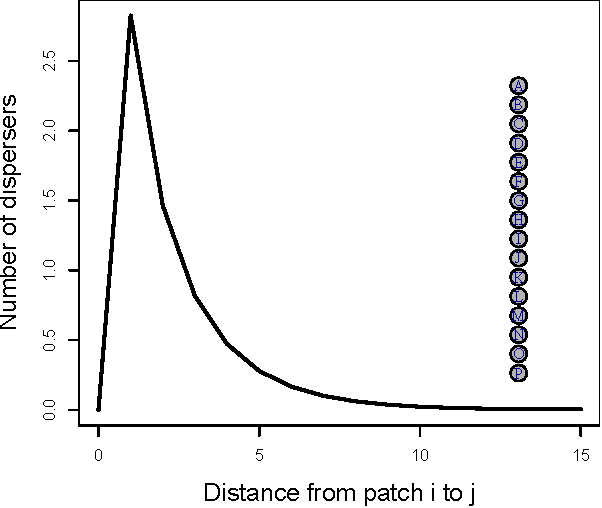
\includegraphics{Managing_for_ecological_surprises_in_metapopulations_files/figure-latex/dispersal-1} 

}

\caption{Example dispersal patterns across linear network.}\label{fig:dispersal}
\end{figure}

\hypertarget{disturbance-regimes}{%
\subsubsection{Disturbance regimes}\label{disturbance-regimes}}

In all scenarios, disturbance was applied after \texttt{50} years of
equilibrating the metapopulation at pristine conditions. We then applied
a pulsed disturbance regime at year \texttt{50} (the regime varied from
\emph{uniform}, \emph{localized, even}, and \emph{localized, uneven} -
see \emph{Scenarios} below). Disturbance immediately removed a fixed
proportion of the metapopulation adults at that time (i.e., \texttt{0.9}
of \(A_{t=50}\)). Once applied, the metapopulation was no longer
disturbed and spatio-temporal recovery dynamics emerged from these
conditions given the ecological scenarios of network complexity,
dispersal rate, spatio-temporal correlations, local patch demographies,
and magnitude of stochastic variance.

\begin{figure}[H]

{\centering 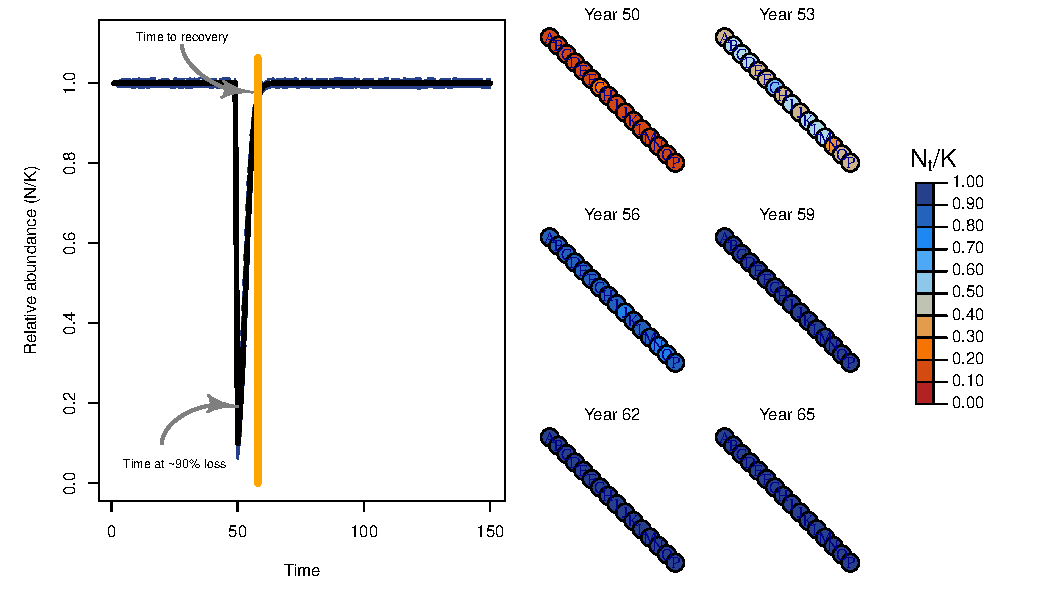
\includegraphics{Managing_for_ecological_surprises_in_metapopulations_files/figure-latex/example disturbance regime-1} 

}

\caption{Recovery regime of metapopulation with linear topology through time (a) and space (b).}\label{fig:example disturbance regime}
\end{figure}

\hypertarget{recruitment-stochasticity}{%
\subsubsection{Recruitment
stochasticity}\label{recruitment-stochasticity}}

Our model allowed for stochastic recruitment that followed a lognormal
distribution with average variation in recruitment of \(\sigma_R\). In
cases with stochastic recruitment, the deterministic recruitment in eq.
S.4 becomes:

\begin{align}
R_{i,t}=\cfrac{\alpha_iN_{i,t-1}}{1+\cfrac{\alpha_i-1}{\beta_i}N_{i,t-1}}e^{(\epsilon_{i,t}-\cfrac{\sigma_{R}^2}{2})}
\end{align}

where lognormal deviates for each patch \emph{i} at time \emph{t} were
drawn from a multivariate normal distribution (\emph{MVN}) with bias
correction \(\cfrac{\sigma_{R}^2}{2}\). If \(\sigma_R\) was low, then
metapopulation dynamics approach the deterministic case. In some
scenarios, we evaluated the role of spatially and/or temporally
correlated deviates among local patches to model potential common
drivers affecting metapopulation dynamics (e.g., Moran effects).
Expected recruitment deviates followed a first-order autoregression
model such that:

\begin{align}
\epsilon_{i,t}=\rho_T\epsilon_{t-1}+MVN(\mu=0,\Sigma=\sigma_R^2(1-\rho_T^2)e^{(-\rho_SD_{i,j})})
\end{align}

where \(\rho_T\) was temporal correlation (bounded \(0-1\)) and
\(\rho_S\) was rate of distance-decay in spatial correlation (bounded
\(0-\infty\) with higher values leading to independent patches). If
\(\rho_T\) was 0 and \(\rho_S\) was high, then annual recruitment
deviates were independent. We modelled the initial conditions for
autoregressive recruitment deviates \(\epsilon_{i,1}\) by drawing from a
stationary normal distribution with mean \(\mu=0\) and variance
\(\sigma_R^2\) such that: \begin{align}
\epsilon_{i,1} \sim N(\mu=0,\sigma=\sigma_R)
\end{align} We illustrate the effects of four kinds of recruitment
deviates below using the same random number generator seed:

\begin{figure}[H]

{\centering 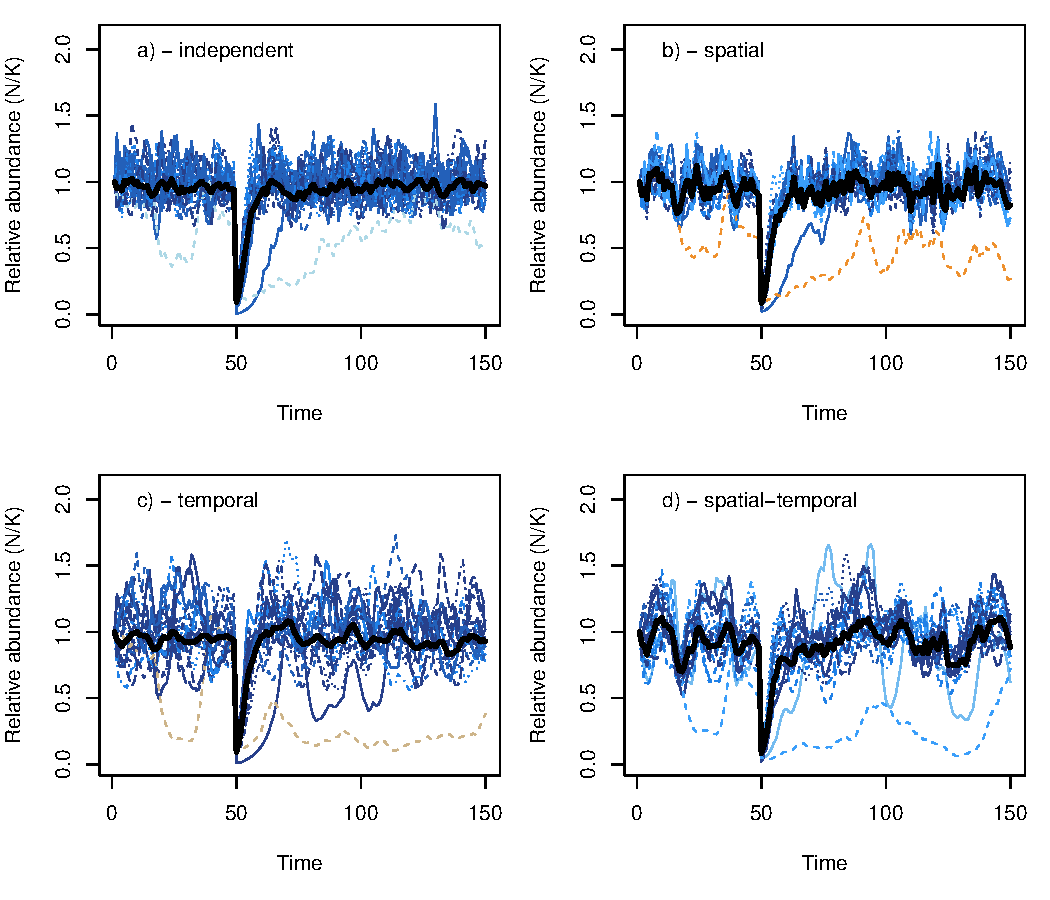
\includegraphics{Managing_for_ecological_surprises_in_metapopulations_files/figure-latex/independent stochasticity-1} 

}

\caption{Metapopulation dynamics with independent (a), spatially correlated (b), temporally correlated (c), and spatio-temporally correlated (d) recruitment deviates. Black line indicates metapopulation, and dashed lines indicate local patches with red and blue relating to abundances after 100 years post-disturbance were less than or greater than 1.0 pre-disturbance, respectively.}\label{fig:independent stochasticity}
\end{figure}

\hypertarget{post-disturbance-outcomes}{%
\subsection{Post-disturbance outcomes}\label{post-disturbance-outcomes}}

\hypertarget{monitoring-management-at-aggregate-scale}{%
\subsubsection{Monitoring \& management at
aggregate-scale}\label{monitoring-management-at-aggregate-scale}}

While true metapopulation dynamics emerge from local patch dynamics and
dispersal in eq. S.1, natural resource managers often monitor and manage
at the scale of the metapopulation. Hence, management at this scale
inherently defines the stock-recruitment dynamics of the aggregate
complex of patches (i.e., metapopulation) as:

\begin{align}
{\mathop{\mathrm{\mathbb{E}}}(N_t)}=\cfrac{\bar{\alpha}{A}_{t-1}}{1+\cfrac{\bar{\alpha}-1}{\bar{\beta}}{A}_{t-1}}
\end{align}

where \(\bar{\alpha}\) was the compensation ratio averaged across the
metapopulation and \(\bar{\beta}\) was the carrying capacity summed
across the entire metapopulation.

\hypertarget{recovery-metrics}{%
\subsubsection{Recovery metrics}\label{recovery-metrics}}

We measured the following post-disturbance outcomes to track the
temporal and spatial recovery regime of the metapopulation.

\begin{enumerate}
\def\labelenumi{\arabic{enumi}.}
\item
  Recovery rate after disturbance: Recovery rate represents the
  proportional post-disturbance recovery towards metapopulation carrying
  capacity gained per year (1 year = 1 generation in our models).
  Recovery rate was calculated as \(1-T_{recovery}/T_{sim}\) where the
  recovery time, \(T_{recovery}\), was the number of years/generations
  it took for the metapopulation to reach five consecutive years ≥
  pre-disturbance abundance. Recovery rate captures how quickly the
  aggregate metapopulation recovers from disturbance but doesn't take
  into account whether any given local patches recover to their
  pre-disturbance capacity nor did it allow for any uncertainty around
  recovery criteria.
\item
  Patch occupancy: The mean number of patches with
  \texttt{\textgreater{}0.1} local carrying capacity after disturbance
  in the short-term (5 years), medium-term (10 years), and long-term (25
  years). This value characterizes the expected risk of spatial
  contractions or local patch collapses, and reflects how interactions
  between spatial structure, disturbance, and dispersal shape
  source-sink dynamics and the ability to provide (or not) rescue
  effects and recover local patches.
\item
  Relative production: The ratio between the empirical metapopulation
  adult abundances to the expected adult recruitment if the
  metapopulation were a single, contiguous population of equivalent size
  and productivity (i.e., carrying capacities and productivity were
  equal to the sum \(\beta\) and mean \(\alpha\) among patches,
  respectively). We term \(\Delta_{N}\) by calculating the
  stock-recruitment model to aggregate metapopulation adults (eq. S.10)
  such that:\\
  \begin{align}
  \Delta_{N_t}=\cfrac{A_t}{\mathop{\mathrm{\mathbb{E}}}(N_t)}
  \end{align}\\
  A value of 1.0 would indicate that the disturbed metapopulation
  production was equal to a single, contiguous population such that
  source-sink dynamics were not consuming surplus recruits. In other
  words, this metric can describe whether the metapopulation acts more
  than (\(\Delta_{N_t}\)\textgreater1.0), less than
  (\(\Delta_{N_t}\)\textless1.0), or equal to the sum of its parts
  (\(\Delta_{N_t}\)=1.0).
\item
  Risk of non-recovery after disturbance: Non-recovery rate was defined
  as the \% of simulations where metapopulation abundance failed to
  recover to \texttt{1.0} of the average pre-disturbance abundance for
  \texttt{5} consecutive years post-disturbance. This ``non-recovery
  rate'' reflects the risk of a long-term state shift in metapopulation
  dynamics after disturbance in the face of stochasticity.
\end{enumerate}

\hypertarget{scenarios}{%
\subsection{Scenarios}\label{scenarios}}

We tested all combinations of the following eight processes (below) and
ran \texttt{100} stochastic iterations per scenario (see section on
\emph{Sensitivity test of mean recovery metrics} below) to estimate the
mean outcome for each of the above recovery metrics:

\begin{enumerate}
\def\labelenumi{\arabic{enumi}.}
\item
  Homogenous and spatially variable recruitment compensation ratio
  across patches, i.e.~intrinsic rate of population growth
  (\(\alpha_i\)).

  \begin{enumerate}
  \def\labelenumii{\alph{enumii}.}
  \tightlist
  \item
    when \emph{variable},
    \(\alpha_i \sim TN(\mu=\bar{\alpha}, \sigma_{\alpha}=0.3\bar{\alpha})\)
    with a truncation applied such that \(5 \leq \alpha_i \geq 1\) to
    ensure that patches could, at minimum, could replace themselves but
    with an upper limit of a 5-fold improvement to per-capita
    productivity. By comparison, Myers et al. (1999) found that
    compensation ratio (their \(\hat\alpha\)) ranged 1-7 for most fish
    species. Since our focus was on at-risk species, we opted to
    truncate this range towards the lower limit, with a mean of
    \texttt{2.0}.
  \end{enumerate}
\item
  Homogenous and spatially variable local carrying capacity across
  patches, i.e.~asymptote of expected recruits at high adult densities
  (\(\beta_i\))

  \begin{enumerate}
  \def\labelenumii{\alph{enumii}.}
  \tightlist
  \item
    when \emph{variable}, \(\beta_i \sim multinomial(p_i,N)\) where
    \(p_i=\cfrac{e^{\theta_i}}{ \sum{e^{\theta_i}}}\),
    \(\theta_i \sim uniform(0,1)\), and \(N=\bar{\beta}\) - with the
    added constraint that \(\beta_i<0.1\bar{\beta}\) to ensure that no
    one patch exceed 10\% of total metapopulation abundance (a necessary
    constraint when modelling \emph{local, even} and \emph{local,
    uneven} disturbances below). \textbf{Note} that, when local
    variation in demography rates occurred, the truncated normal in
    \emph{Appendix S1: Section 1.3.1.a} and truncated multinomial in
    \emph{Appendix S1: Section 1.3.2.a} above led compensation ratio and
    carrying capacity, respectively, to vary by the same magnitude
    \textasciitilde28\% coefficient of variation (Appendix S1: Figure
    S6).
  \end{enumerate}
\item
  Disturbances where a proportion of individuals removed from
  metapopulation (e.g., \texttt{0.90}) occurs.

  \begin{enumerate}
  \def\labelenumii{\alph{enumii}.}
  \tightlist
  \item
    \emph{uniform} - random individuals removed at equal vulnerability
    across all patches.
  \item
    \emph{local, even} - random individuals removed from randomly
    selected subset of patches (as long as the target individuals lost
    in the metapopulation can be achieved in that subset of patches)

    \begin{enumerate}
    \def\labelenumiii{\roman{enumiii}.}
    \tightlist
    \item
      Specifically, a numerical algorithm was used to search and find a
      set of disturbance conditions whereby removing a random proportion
      of individuals from a random subset of local patches achieved
      both:

      \begin{itemize}
      \tightlist
      \item
        total loss summed to a \textasciitilde90\% loss in abundance to
        the whole metapopulation, and
      \item
        left at least one local patch \emph{undisturbed} to start
        metapopulation recoveries.
      \end{itemize}
    \end{enumerate}
  \item
    \emph{local, uneven} - total extirpation of randomly selected subset
    of patches (as long as the target individuals lost in the
    metapopulation can be achieved in that subset of patches).

    \begin{enumerate}
    \def\labelenumiii{\roman{enumiii}.}
    \tightlist
    \item
      Specifically, a numerical algorithm was used to search and find a
      set of local demographic conditions whereby extirpations to a
      random subset of local patches that achieved both:

      \begin{itemize}
      \tightlist
      \item
        total loss summed to a \textasciitilde90\% loss in abundance to
        the whole metapopulation, and
      \item
        left at least one local patch \emph{undisturbed} to start
        metapopulation recoveries.
      \end{itemize}
    \end{enumerate}
  \end{enumerate}
\item
  Density-independent dispersal rates \(\omega\) from 0 to 5\% of
  individuals within a patch will disperse.
\item
  Topology of the spatial networks with linear, dendritic, star, and
  grid networks. Each network with \(P=16\) and distance between patches
  \(\bar{d}=1\).
\item
  Stochastic recruitment deviates with low, medium, and high standard
  deviation in lognormal error. Used to generate stochastic population
  dynamics via random deviates from the expected recruitment
  relationship in eq. S.2.
\item
  Temporal correlation in recruitment deviates from low, medium, and
  high correlation (i.e., good year at time \emph{t} begets good year at
  time \emph{t+1}).
\item
  Spatial correlation in recruitment deviates among patches from low,
  medium, to high correlation (i.e., neighboring patches go up or down
  together).
\end{enumerate}

\begin{figure}[H]

{\centering 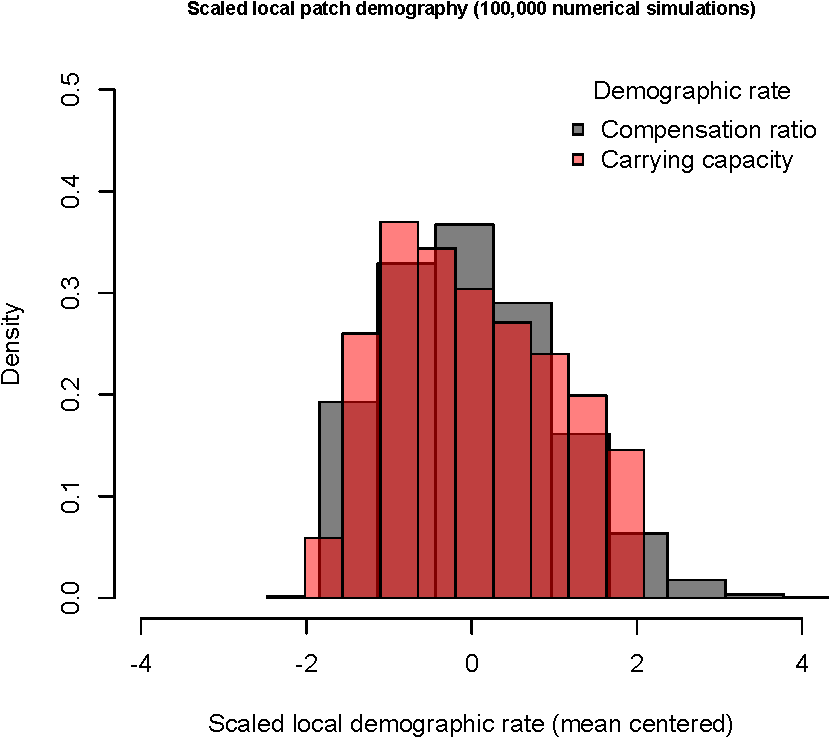
\includegraphics{Managing_for_ecological_surprises_in_metapopulations_files/figure-latex/histogram of demographic variation-1} 

}

\caption{Histogram showing variation among demographic rates after simulatng 100,000 local patches when using the truncated normal in Appendix S1: Section 1.3.1.a and truncated multinomial in Appendix S1: Section 1.3.2.a when modelling variation in local compensation ratio (grey) and carrying capacity (red).}\label{fig:histogram of demographic variation}
\end{figure}

\hypertarget{example-results}{%
\subsubsection{Example results}\label{example-results}}

We demonstrate our metapopulation model with an example outcome for a
linear network composed of \texttt{16} patches, a dispersal rate of
\texttt{0.01} and a high enough dispersal cost such that individuals are
only willing to move to their closest neighboring patches. This limits
the strength of potential rescue effects. For this example, patches
varied in their productivity and carrying capacity but will have
deterministic population dynamics.

\begin{figure}[H]

{\centering 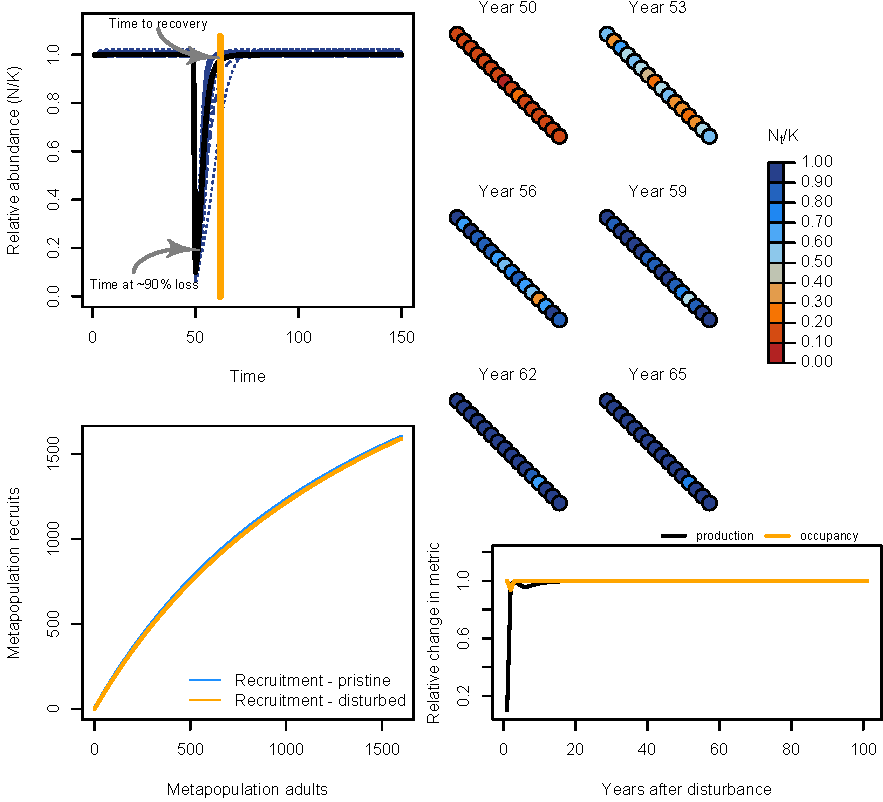
\includegraphics{Managing_for_ecological_surprises_in_metapopulations_files/figure-latex/example results1-1} 

}

\caption{Example iteration of spatial recovery regime of metapopulation with linear topology through time (top left) and space (top right). Recruitment dynamics before and 10 years after disturbance (bottom left). Relative bias in aggregate-scale estimates of carrying capacity, compensation ratio, and recruitment production in recovery phase (bottom right).}\label{fig:example results1}
\end{figure}
\newpage

We can then contrast this with a different network shape, like a
dendritic network.

\begin{figure}[H]

{\centering 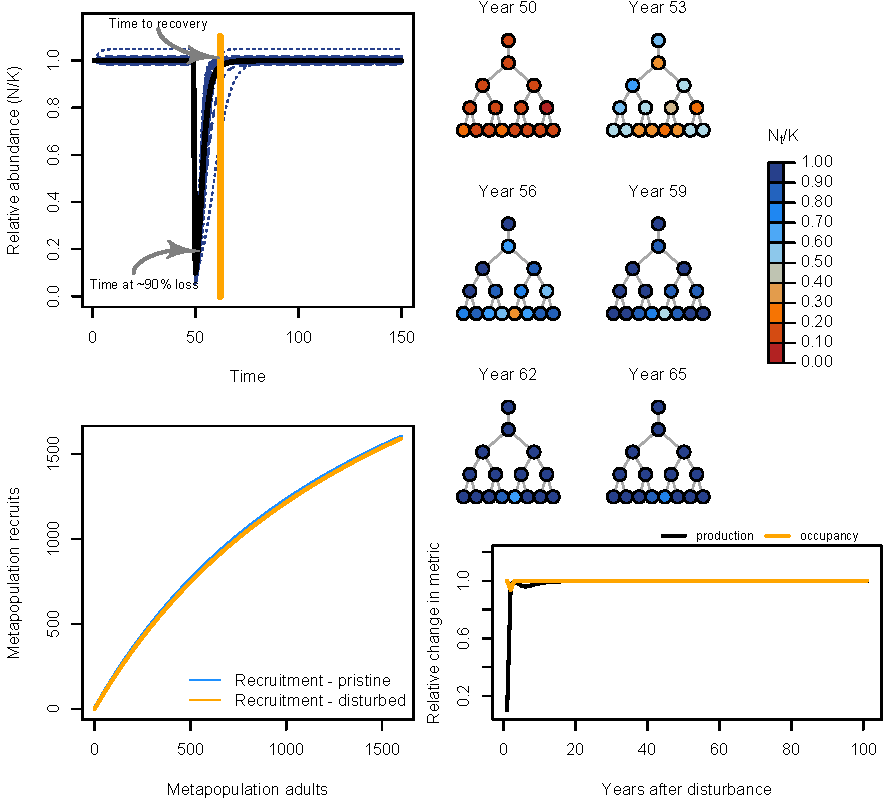
\includegraphics{Managing_for_ecological_surprises_in_metapopulations_files/figure-latex/example results2-1} 

}

\caption{Example iteration of spatial recovery regime of metapopulation with dendritic topology.}\label{fig:example results2}
\end{figure}
\newpage

Now, let's add some stochasticity to recruitment and see how this
affects the recovery regime.

\begin{figure}[H]

{\centering 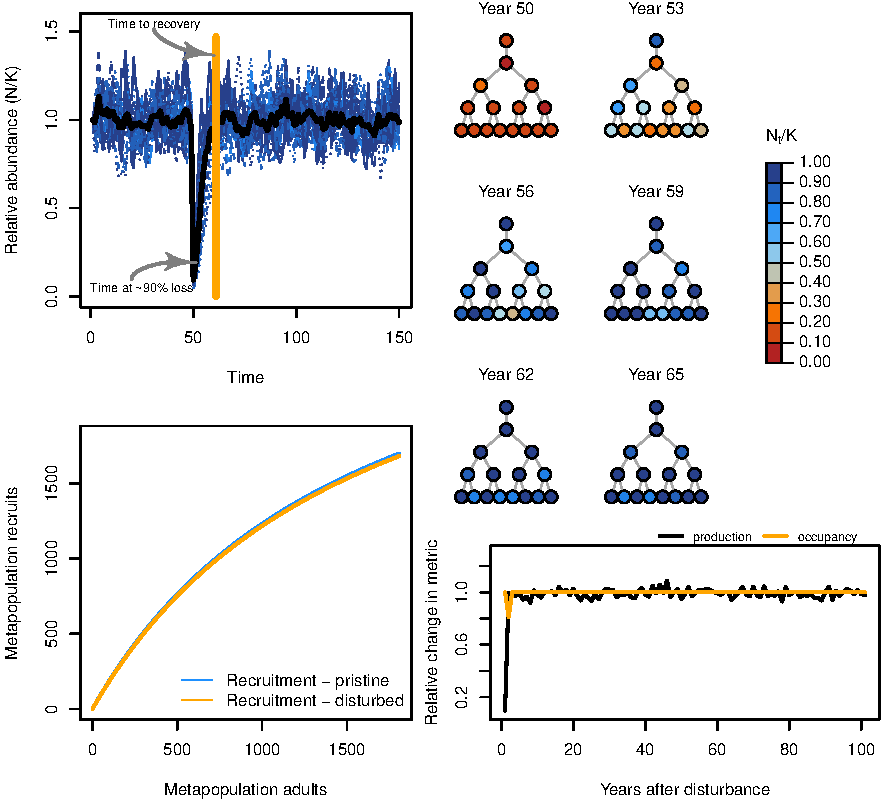
\includegraphics{Managing_for_ecological_surprises_in_metapopulations_files/figure-latex/example results3-1} 

}

\caption{Example iteration of spatial recovery regime of stochastic metapopulation.}\label{fig:example results3}
\end{figure}
\newpage

Next, we can contrast with a disturbance regime where the disturbance is
concentrated on local patches that can be completely extirpated (rather
than the disturbance being applied proportionally across all patches
e.g., a mixed-stock fishery).

\begin{figure}[H]

{\centering 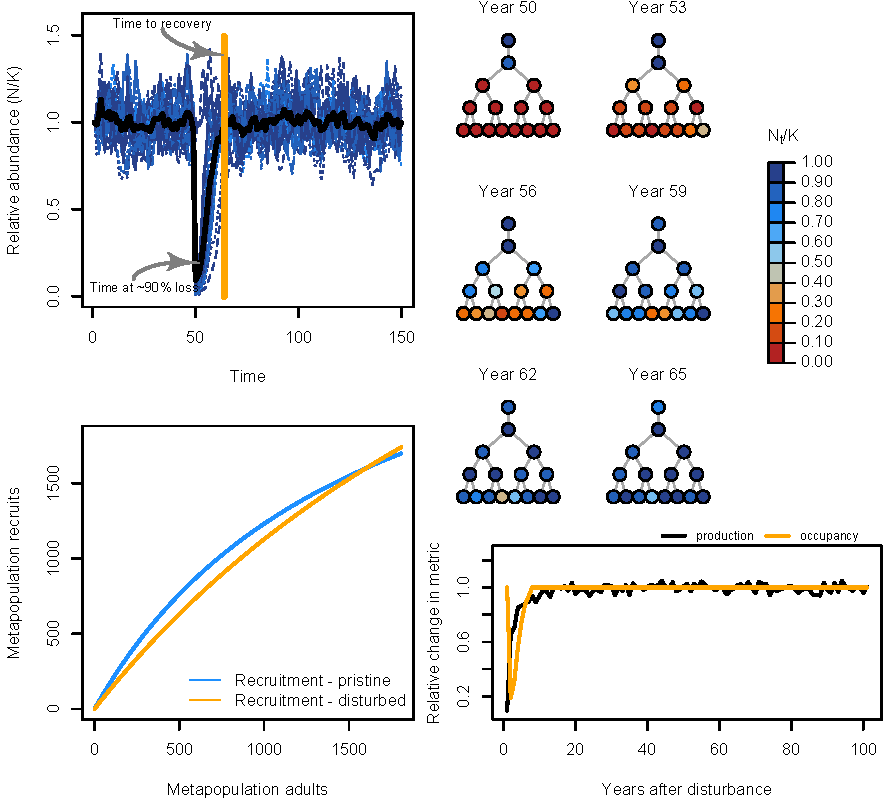
\includegraphics{Managing_for_ecological_surprises_in_metapopulations_files/figure-latex/example results4-1} 

}

\caption{Example iteration of spatial recovery regime of stochastic metapopulation.}\label{fig:example results4}
\end{figure}
\newpage

\hypertarget{sensitivity-test-of-mean-recovery-metrics}{%
\subsection{Sensitivity test of mean recovery
metrics}\label{sensitivity-test-of-mean-recovery-metrics}}

The total number of scenarios resulted in a long computation time to run
all simulations a large number of times necessary to evaluate how
metapopulation responded, on average, to our ecological and disturbance
scenarios. To determine a sufficient number of bootstrap iterations to
run, we ran a sensitivity test to explore the relative sensitivity of
the mean for a few recovery metrics of interest (recovery rate) to the
number of stochastic simulations ran per scenario. Below, we repeated
the scenario for a metapopulation with a dendritic network, with high
stochasticity, locally uneven disturbances, large spatial-temporal
correlations, variable patch productivities, and variable patch
capacities along gradients of 10, 100, 500, and 1,000 stochastic
simulations. Based on these preliminary results, we see that the mean
for most metrics was relatively insensitive with at least 100
simulations.

\begin{figure}[H]

{\centering 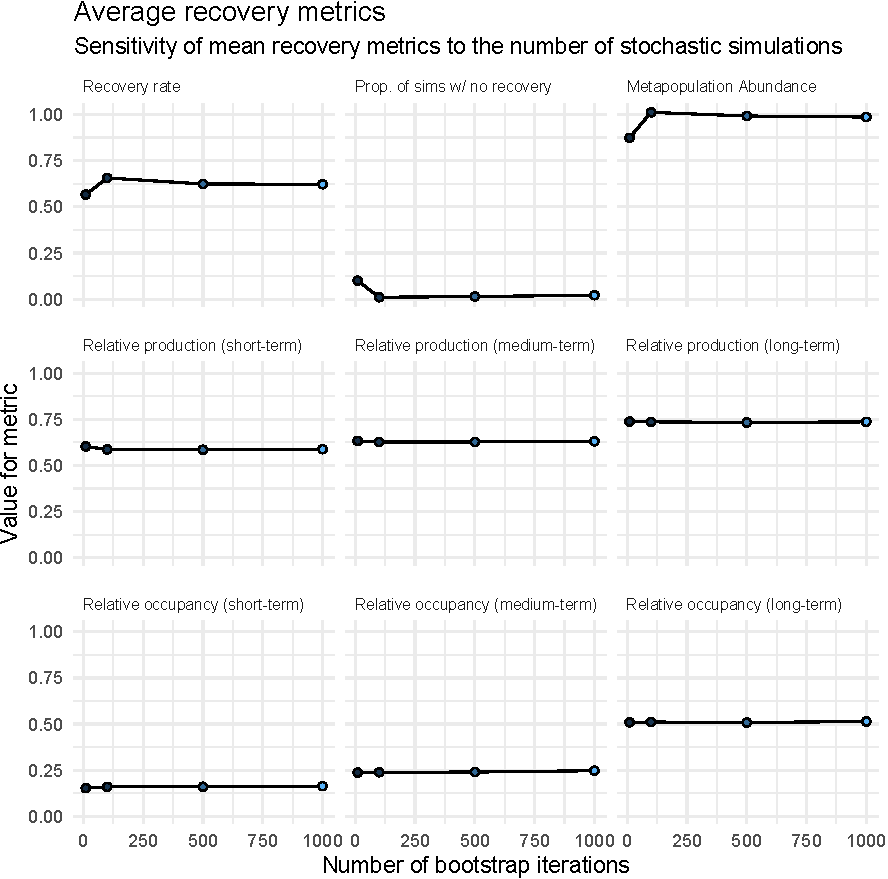
\includegraphics{Managing_for_ecological_surprises_in_metapopulations_files/figure-latex/bootstrap results-1} 

}

\caption{Sensitivity test of mean recovery metrics to number of iterations to bootstrap the stochastic simulations. Example metapopulation consisted of a dendritic network, high recruitment stochasticity, locally uneven disturbance regime, large spatial-temporal correlations, variable patch productivities, and variable patch capacities tested along gradients of 10, 100, 500, and 1,000 bootstrapped iterations.}\label{fig:bootstrap results}
\end{figure}
\newpage

\hypertarget{general-patterns}{%
\subsection{General patterns}\label{general-patterns}}

\hypertarget{effects-of-disturbance-regime}{%
\subsubsection{Effects of disturbance
regime}\label{effects-of-disturbance-regime}}

The strongest lever influencing recovery in our simulated
metapopulations was, by far, the characteristics of the disturbance
regime. Specifically, the degree to how locally concentrated the
disturbance was on the set of patches was more influential than variable
density dependence, dispersal rates, or network topology. Localized
disturbances increased the risk of spatial contraction, reduced recovery
rates and aggregate compensation, and increased the risk of
non-recoveries. By altering aggregate compensation, localized
disturbance reduced the relative production of the metapopulation. In
other words, through changes in source-sink dynamics, metapopulations
under localized disturbance acted less than the sum of their parts --
the more localized the impacts, the worse these effects. Uniform
disturbances generally left the metapopulation dynamics unaffected with
few changes to recovery metrics outside of occasionally slower
recoveries. These above spatial and temporal recovery processes also
appeared tied to one another such that changes to any of them had
feedbacks with other recovery metrics. Perhaps intuitively, for example,
patch occupancy was highly correlated to the relative production of the
metapopulation, such that the more patches occupied, the more that
metapopulation dynamics resembled a contiguous population.

\begin{figure}[H]

{\centering 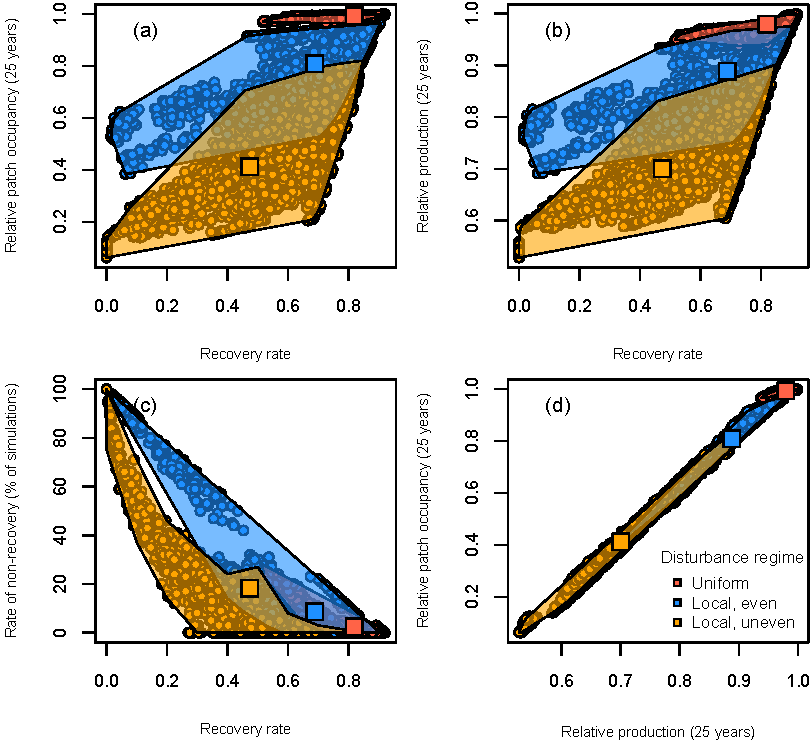
\includegraphics{Managing_for_ecological_surprises_in_metapopulations_files/figure-latex/disturbance regime-1} 

}

\caption{The role of spatial disturbance regimes on metapopulation recoveries and covariation among four recovery metrics: (a,b,c) recovery rate – the annual rate of metapopulation recovery; (a,d) relative patch occupancy – the mean proportion of patches occupied 25 years after disturbance; (b,d), relative production – the ratio between the summed abundances across all patches to the expected production of an equivalent single population 25 years after disturbance; and (c) rate of non-recovery – the percent of 100 stochastic simulations where the metapopulation failed to recover. Each point represents a single simulation for a metapopulation under a unique combination of local productivity, dispersal, spatial network, stochasticity, and disturbance (9,504 total simulations). Shaded regions describe the range in recovery metrics for all simulated metapopulations and are colored by disturbance regime. Square points represent the mean recovery metrics from all simulations within each disturbance regime.}\label{fig:disturbance regime}
\end{figure}
\newpage

\hypertarget{role-of-network-structure-dispersal}{%
\subsubsection{Role of network structure \&
dispersal}\label{role-of-network-structure-dispersal}}

We now show some general patterns in how variable patch demographic
rates, network structure, dispersal, disturbance, recruitment
stochasticity, and spatio-temporal correlations variation affects
metapopulation \emph{recovery rates} (shown in Figure 4 of the main text
and Figure S13), \emph{non-recovery rate} (i.e, the number of
simulations where the metapopulation fails to recover; Figure S14),
\emph{patch occupancy} (i.e., number of patches with local abundance
\textless10\% of pre-disturbance; Figure S15), and \emph{relative
production} (Figure S16).

\begin{figure}[H]

{\centering 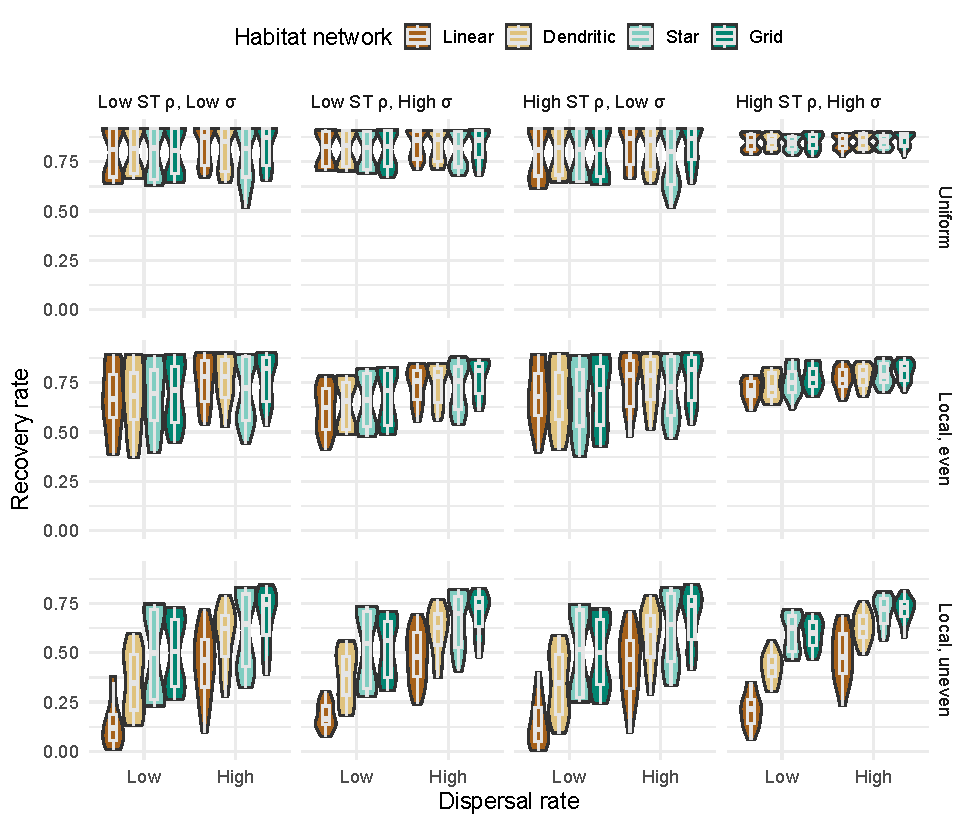
\includegraphics{Managing_for_ecological_surprises_in_metapopulations_files/figure-latex/violin plots of risk of recovery rates-1} 

}

\caption{Violin plots showing marginal response of metapopulation recovery rates along gradients of network configuration, dispersal categories (low≤0.001; high>0.001), spatial-temporal (ST) correlations (low $\rho$≈0; high $\rho$=0.6), scale of lognormal variance in recruitment (low $\sigma$= 0.001; high $\sigma$=0.1), and spatial distribution of disturbance.}\label{fig:violin plots of risk of recovery rates}
\end{figure}

Next, we show violin plots demonstrating some of the modulating factors
leading to variation in the risk of non-recovery owing to stochastic
recruitment dynamics.

\begin{figure}[H]

{\centering 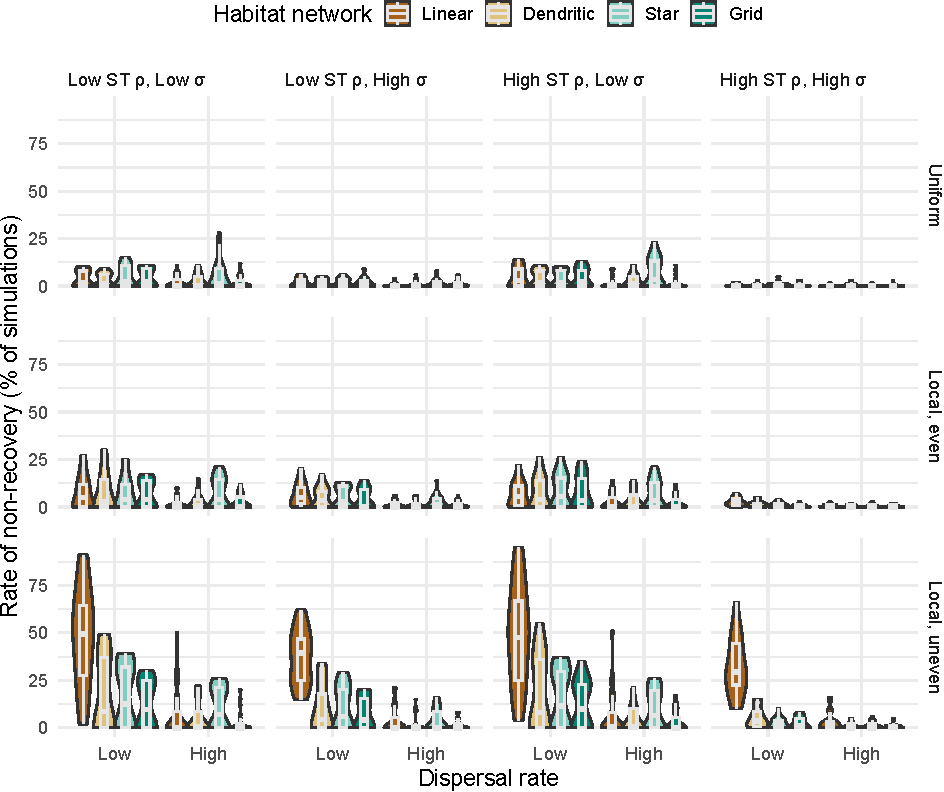
\includegraphics{Managing_for_ecological_surprises_in_metapopulations_files/figure-latex/violin plots of risk of non-recovery-1} 

}

\caption{Violin plots showing marginal response of the stochastic risk of non-recovery in metapopulations along gradients of network configuration, dispersal categories (low≤0.001; high>0.001), spatial-temporal (ST) correlations (low $\rho$≈0; high $\rho$=0.6), scale of lognormal variance in recruitment (low $\sigma$= 0.001; high $\sigma$=0.1), and spatial distribution of disturbance.}\label{fig:violin plots of risk of non-recovery}
\end{figure}

Next, we show violin plots demonstrating some of the modulating factors
leading to variation in long-term impacts to patch occupancy.

\begin{figure}[H]

{\centering 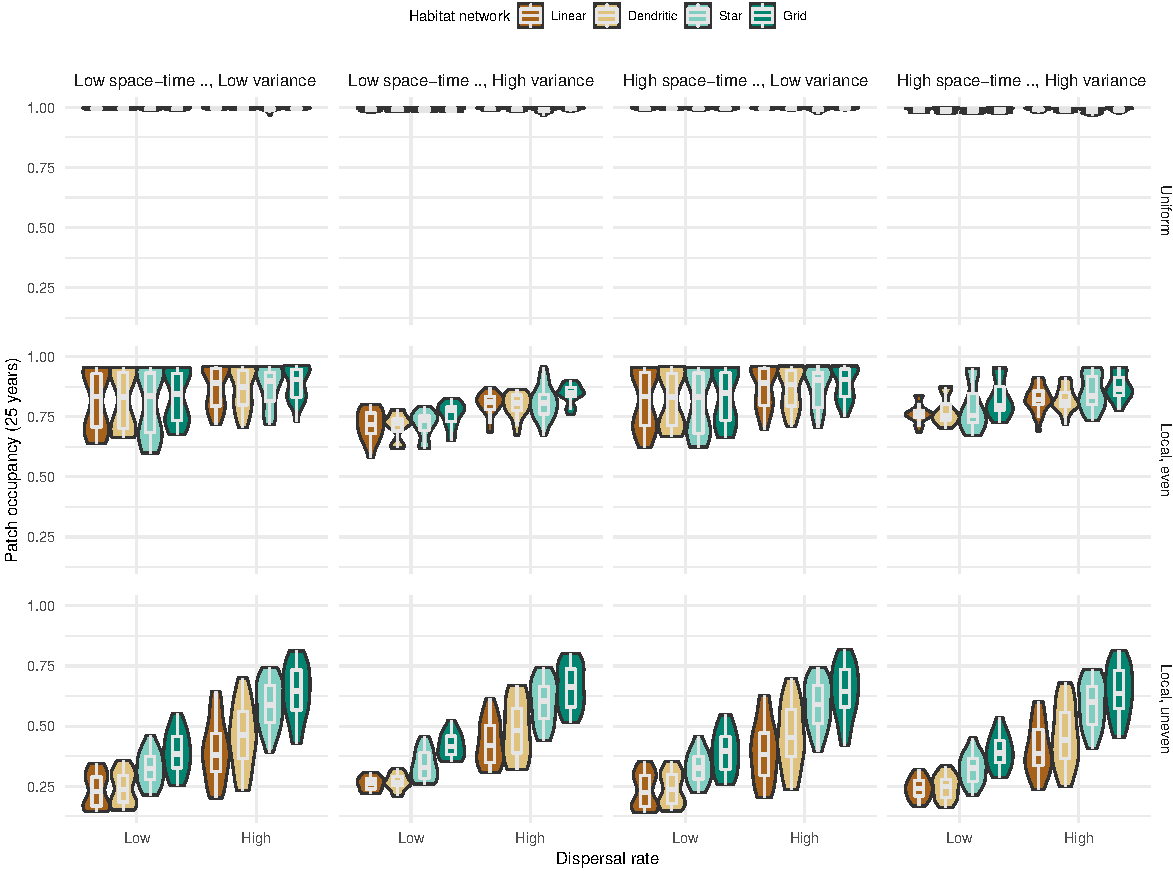
\includegraphics{Managing_for_ecological_surprises_in_metapopulations_files/figure-latex/violin plots of risk of patch occupancy-1} 

}

\caption{Violin plots showing marginal response of long-term patch occupancy in metapopulations along gradients of network configuration, dispersal categories (low≤0.001; high>0.001), spatial-temporal (ST) correlations (low $\rho$≈0; high $\rho$=0.6), scale of lognormal variance in recruitment (low $\sigma$= 0.001; high $\sigma$=0.1), and spatial distribution of disturbance.}\label{fig:violin plots of risk of patch occupancy}
\end{figure}

Next, we show variation in relative production metrics. Figure S12 shows
the tight correlation between patch occupancy and relative production.
Hence, Figure S15 and S16 look quite similar.

\begin{figure}[H]

{\centering 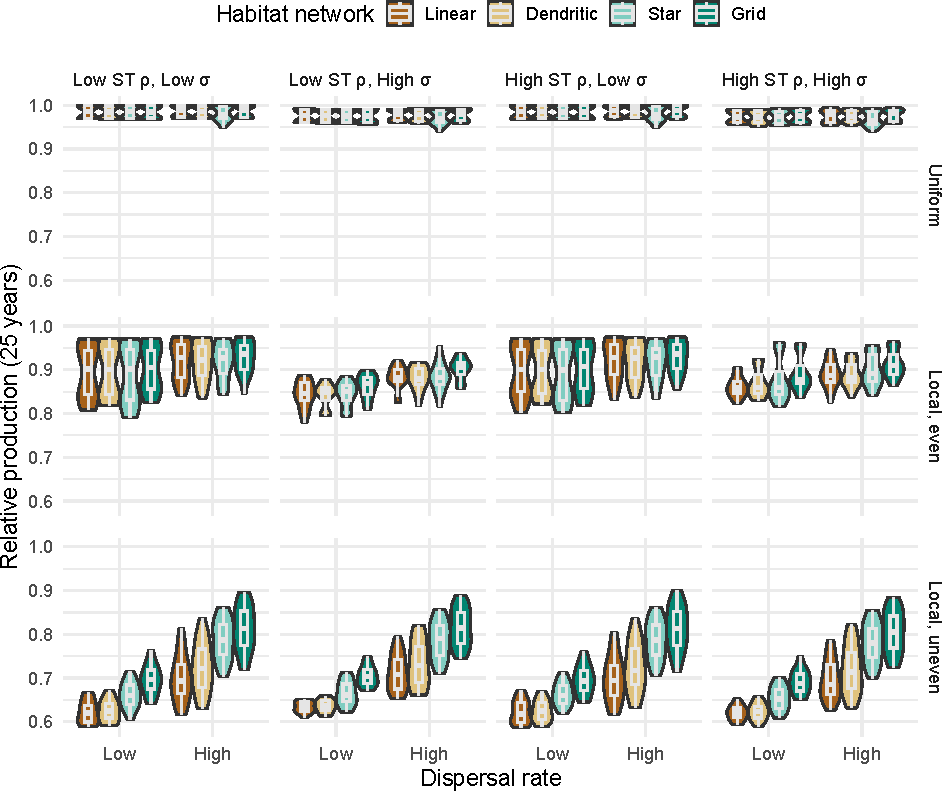
\includegraphics{Managing_for_ecological_surprises_in_metapopulations_files/figure-latex/violin plots of risk of relative production-1} 

}

\caption{Violin plots showing marginal response of relative production for metapopulations along gradients of network configuration, dispersal categories (low≤0.001; high>0.001), spatial-temporal (ST) correlations (low $\rho$≈0; high $\rho$=0.6), scale of lognormal variance in recruitment (low $\sigma$= 0.001; high $\sigma$=0.1), and spatial distribution of disturbance.}\label{fig:violin plots of risk of relative production}
\end{figure}

Dispersal, landscape structure, and local density-dependence also
affected metapopulation recovery patterns in three key ways, though to a
lesser extent. First, recovery rates increased with increased dispersal.
However, this effect was nonlinear with diminishing benefits of
dispersal occurring at \textasciitilde1-3\%, depending on spatial
structure and disturbance. Second, more linearized networks had slower
recovery times than more connected networks suggesting that rescue
effects take some time to cascade through the entire network of patches;
but this interacted with the disturbance regime as only local,
extirpation exhibited this change in any substantial manner. Last,
diversity in local patch compensation and carrying capacities tended to
slow metapopulation recoveries - this effect interacted with other
factors like stochasticity.

\newpage

\hypertarget{clustering-analyses}{%
\subsubsection{Clustering analyses}\label{clustering-analyses}}

We used hierarchical clustering analyses (implementing Ward's criterion)
of a dissimilarity matrix from our four recovery metrics to evaluate
whether there was evidence for common recovery regimes among our
simulation results across all ecological and disturbance scenarios
(Murtagh \& Legendre 2014). Based on advice laid out in Hennig (2014),
we determined that the best number of unique clusters in metapopulation
recoveries should satisfy the following statistical criteria:

\begin{enumerate}
\def\labelenumi{\arabic{enumi}.}
\tightlist
\item
  recovery outcomes from within a cluster are closer to one another than
  to other clusters (i.e., the two Dunn indices are relatively high)
\item
  the number of clusters explains much of the point variation within the
  dataset (i.e., diminishing returns in minimizing the sums-of-squared
  residuals)
\item
  the point observations within clusters are relatively tight (i.e.,
  both the average silhouette width and the widest within-cluster gap
  are relatively low)
\item
  clusters are relatively unique and there is good separation between
  the clusters (i.e., the separation index is still high, while
  considering that low numbers of clusters should always have the
  highest separation)
\end{enumerate}

\begin{figure}[H]

{\centering 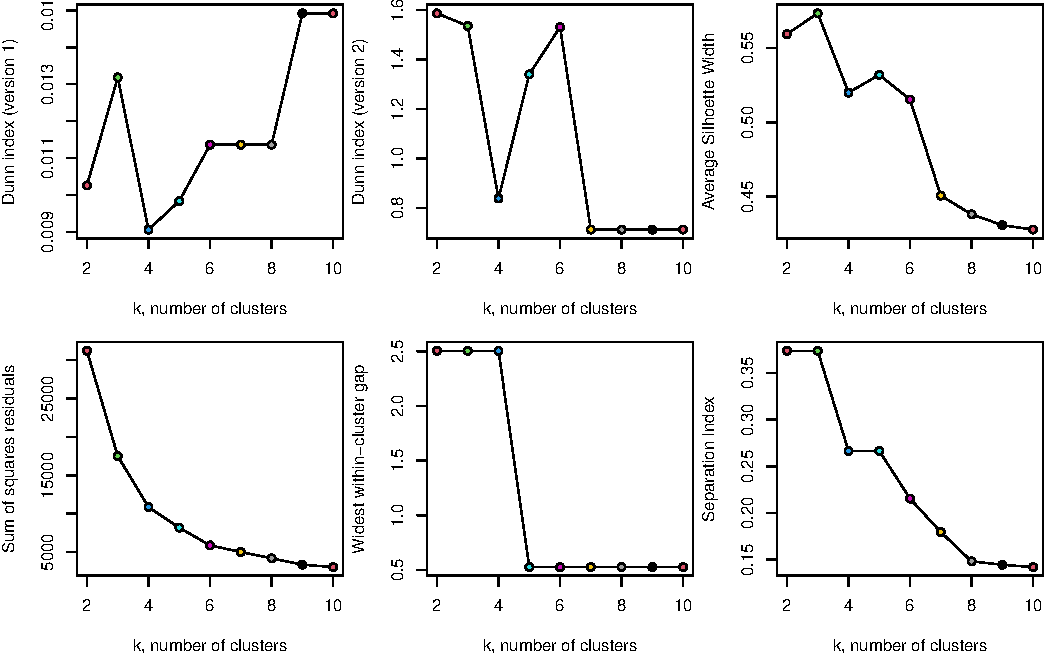
\includegraphics{Managing_for_ecological_surprises_in_metapopulations_files/figure-latex/clustering analysis-1} 

}

\caption{The relationships between number of potential clusters and multiple statistical criteria used to test support for the best number of clusters within the simulated recovery outcomes}\label{fig:clustering analysis}
\end{figure}

Based on the above criteria, we chose 5 unique clusters as satisfying
most of the above criteria in the figure above, although there was good
support for between 3 and 6 unique clusters. The principal components
analysis indicates that five clusters has substantial explanatory power
of metapopulation recovery metrics (explained \textasciitilde89\% of the
point variation).

\begin{figure}[H]

{\centering 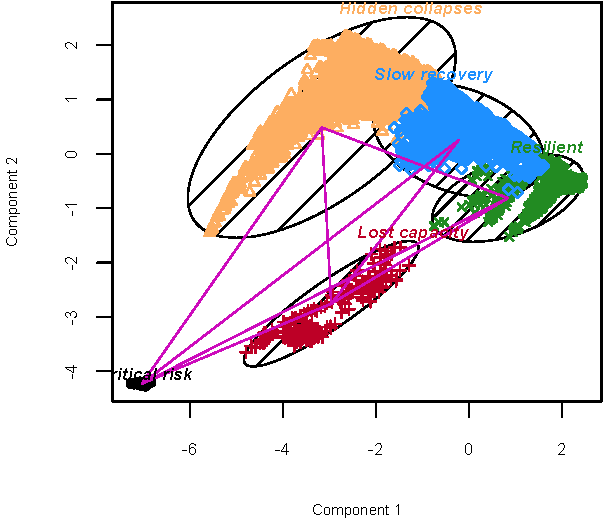
\includegraphics{Managing_for_ecological_surprises_in_metapopulations_files/figure-latex/clustering plot-1} 

}

\caption{Bivariate cluster plot of the principal components explaining point variation in metapopulaton recovery metrics acrosss all simulated scenarios grouped into five distinct clusters.}\label{fig:clustering plot}
\end{figure}

\hypertarget{emergent-recovery-outcomes}{%
\subsubsection{Emergent recovery
outcomes}\label{emergent-recovery-outcomes}}

Overall, we used hierarchical clustering analyses to describe five
common metapopulation recovery outcomes. These outcomes were: (1)
resilient recovery -- metapopulations recovered to pre-disturbance
abundances quickly with all patches occupied, (2) slow recovery --
metapopulation recovery was slow but there were no other changes in
metrics, (3) hidden collapses -- metapopulations tended to recover and
aggregate abundances were high, but many local patches remained
unoccupied and recovery was slowed, (4) lost capacity -- recovery rates
were very slow, the risk of non-recovery was high, long-term production
was low, and many local patches remained unoccupied and (5) critical
risk -- where metapopulations failed to recover, abundances remained
low, and the risk of non-recovery was high.

\begin{longtable}[t]{>{\raggedright\arraybackslash}p{2.75cm}>{\raggedright\arraybackslash}p{1.4cm}>{\raggedright\arraybackslash}p{2.25cm}>{\centering\arraybackslash}p{1.1cm}>{\centering\arraybackslash}p{1.4cm}>{\centering\arraybackslash}p{1.1cm}>{\centering\arraybackslash}p{1.4cm}>{\centering\arraybackslash}p{1.7cm}>{\centering\arraybackslash}p{1.7cm}}
\caption{\label{tab:clustering table}The mean recovery metrics, total sample size per regime (No.), and metapopulation abundance (N/K) for each of five common metapopulation recovery regimes supported by hierarchical clustering analyses across gradients in disturbance and network structure.}\\
\toprule
Regime & Network & Disturbance & No. & Recovery rate & \% non-recovery & Occupancy & Relative production & Relative abundance\\
\midrule
Resilient & Linear & Uniform & 792 & 0.83 & 2 & 0.99 & 0.98 & 1.00\\
Resilient & Dendritic & Uniform & 792 & 0.82 & 2 & 0.99 & 0.98 & 0.99\\
Resilient & Star & Uniform & 792 & 0.81 & 3 & 0.99 & 0.98 & 0.99\\
Resilient & Grid & Uniform & 792 & 0.82 & 2 & 0.99 & 0.98 & 1.00\\
Resilient & Linear & Local, even & 205 & 0.78 & 5 & 0.94 & 0.95 & 0.99\\
Resilient & Dendritic & Local, even & 201 & 0.78 & 5 & 0.94 & 0.96 & 0.99\\
Resilient & Star & Local, even & 274 & 0.75 & 7 & 0.93 & 0.95 & 0.99\\
Resilient & Grid & Local, even & 215 & 0.78 & 5 & 0.94 & 0.96 & 0.99\\
\addlinespace
Slow recovery & Linear & Local, even & 528 & 0.69 & 3 & 0.77 & 0.87 & 0.99\\
Slow recovery & Dendritic & Local, even & 533 & 0.70 & 3 & 0.77 & 0.87 & 0.99\\
Slow recovery & Star & Local, even & 466 & 0.68 & 5 & 0.75 & 0.86 & 0.99\\
Slow recovery & Grid & Local, even & 529 & 0.73 & 3 & 0.81 & 0.89 & 0.99\\
Slow recovery & Linear & Local, uneven & 11 & 0.72 & 0 & 0.64 & 0.81 & 1.00\\
Slow recovery & Dendritic & Local, uneven & 69 & 0.73 & 0 & 0.66 & 0.81 & 0.99\\
Slow recovery & Star & Local, uneven & 114 & 0.74 & 4 & 0.71 & 0.84 & 0.97\\
Slow recovery & Grid & Local, uneven & 244 & 0.76 & 0 & 0.73 & 0.85 & 1.00\\
\addlinespace
Hidden collapses & Linear & Local, even & 9 & 0.61 & 3 & 0.59 & 0.79 & 0.99\\
Hidden collapses & Dendritic & Local, even & 9 & 0.65 & 0 & 0.59 & 0.78 & 0.99\\
Hidden collapses & Star & Local, even & 4 & 0.72 & 0 & 0.55 & 0.76 & 1.00\\
Hidden collapses & Linear & Local, uneven & 709 & 0.34 & 21 & 0.34 & 0.67 & 0.97\\
Hidden collapses & Dendritic & Local, uneven & 651 & 0.49 & 8 & 0.36 & 0.68 & 0.99\\
Hidden collapses & Star & Local, uneven & 606 & 0.57 & 9 & 0.45 & 0.72 & 0.99\\
Hidden collapses & Grid & Local, uneven & 476 & 0.56 & 7 & 0.46 & 0.73 & 0.99\\
\addlinespace
Lost capacity & Linear & Local, even & 50 & 0.17 & 77 & 0.58 & 0.79 & 0.66\\
Lost capacity & Dendritic & Local, even & 49 & 0.16 & 78 & 0.58 & 0.78 & 0.65\\
Lost capacity & Star & Local, even & 48 & 0.16 & 78 & 0.58 & 0.78 & 0.65\\
Lost capacity & Grid & Local, even & 48 & 0.16 & 79 & 0.57 & 0.78 & 0.64\\
\addlinespace
Critical risk & Linear & Local, uneven & 72 & 0.00 & 100 & 0.10 & 0.54 & 0.09\\
Critical risk & Dendritic & Local, uneven & 72 & 0.00 & 100 & 0.10 & 0.54 & 0.08\\
Critical risk & Star & Local, uneven & 72 & 0.00 & 100 & 0.10 & 0.54 & 0.08\\
Critical risk & Grid & Local, uneven & 72 & 0.00 & 100 & 0.10 & 0.54 & 0.08\\
\bottomrule
\end{longtable}

In general, the five recovery regimes spanned a continuum of better
(e.g., resilient) to worse recoveries (e.g., long-term critical risks).
Overall, the interplay between ecological and disturbance conditions
appeared to structure the specific pathway for metapopulation recoveries
(Figure S19; Table S2). For example, uniform disturbances always led to
resilient recoveries. However, local, even disturbance regimes tended to
lead to, at-best, a resilient recovery or, at worst, hidden collapses
with the probability modulated by other ecological factors. Local,
uneven disturbance regimes led to, at best, a slow recovery or, at
worst, a long-term critical risk and non-recovery. The main text Figure
5 and 6 demonstrates the conditions that led to resilient recoveries
compared to critical risks, while more intermediate outcomes, like slow
recovery, hidden collapses, or lost capacity are shown here in Figures
S20-S22.

\begin{figure}[H]

{\centering 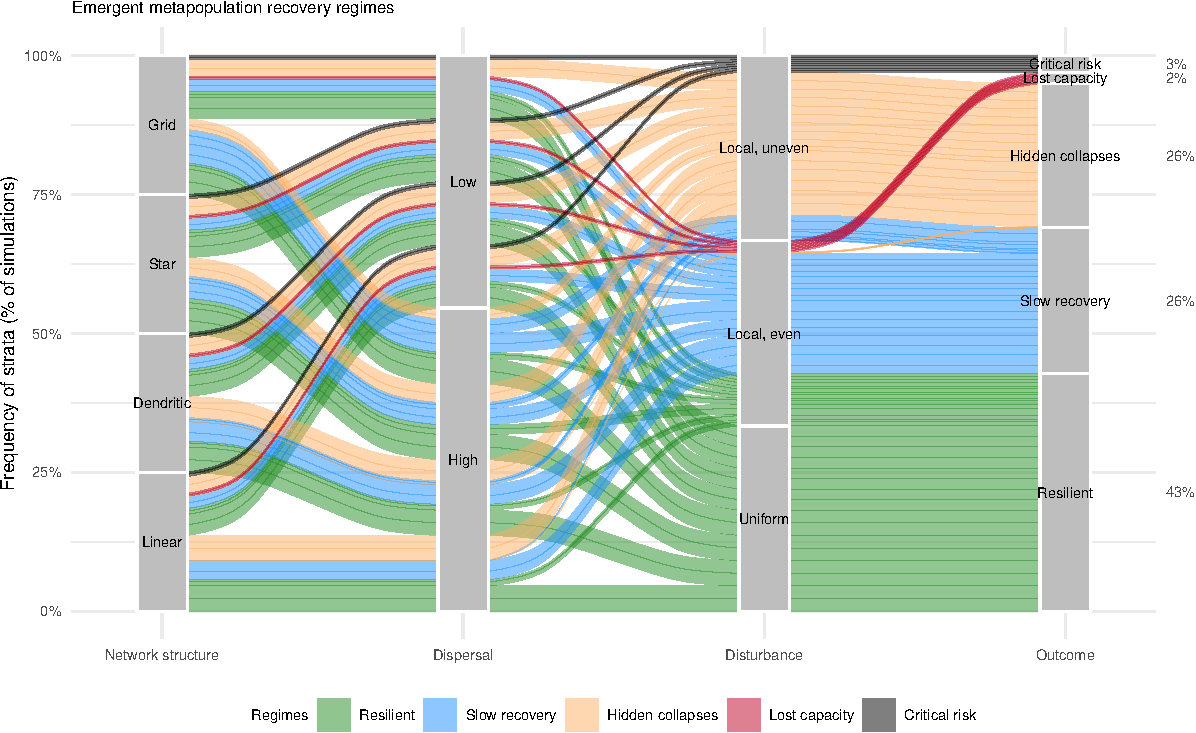
\includegraphics{Managing_for_ecological_surprises_in_metapopulations_files/figure-latex/cluster results-1} 

}

\caption{Frequency of emergent metapopulation recovery regimes can depend on a complex interplay between network structure, dispersal, and spatial disturbances. Ribbon colors denote a group of simulations that led to one of five common recovery outcomes. Frequency of regimes denoted by width of ribbons}\label{fig:cluster results}
\end{figure}

Local patch demography, habitat network structure, dispersal, spatially
and temporally correlated recruitment variation, and spatial disturbance
regimes each had modulating effects on the probability for any
particular recovery regime (Figures 5 \& 6 in the main text; and Figures
S20-S22 here). There was a clear signal from any localized disturbances,
which increased the probability for non-resilient recovery regimes. For
habitat networks, metapopulations with linear networks tended to have
increased probability for worse recoveries compared to gridded networks.
For dispersal rates, metapopulations with low dispersal had increased
probability for poor recoveries compared to high dispersal. For local
demography, metapopulations with variable local patch demographic rates
tended to increased probability for poor recoveries compared to
metapopulations composed of homogeneous local patches. For recruitment
stochasticity, metapopulations with both high recruitment variation and
high spatial-temporal correlations led to increased probability for poor
recoveries compared to low variation and low correlations.

\begin{figure}[H]

{\centering 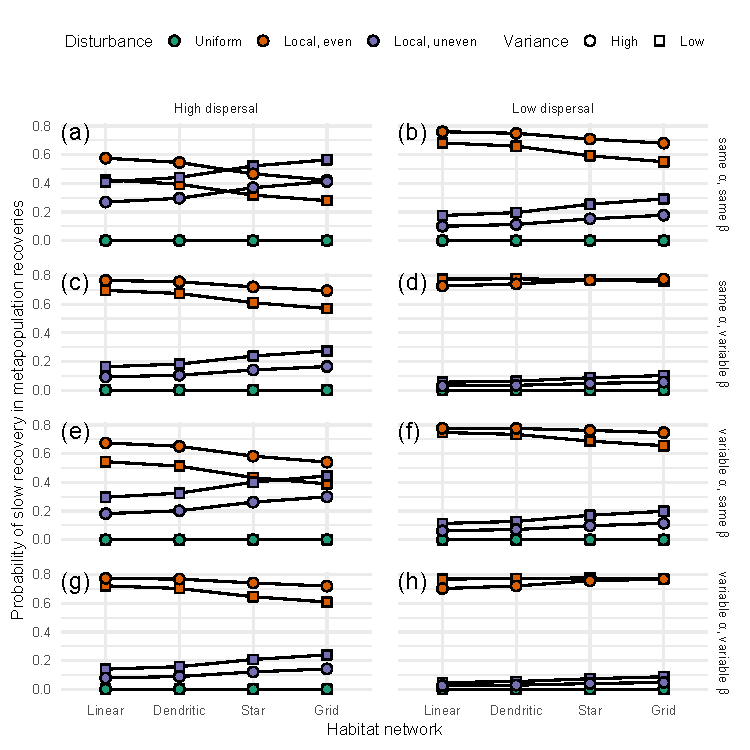
\includegraphics{Managing_for_ecological_surprises_in_metapopulations_files/figure-latex/conditional probability for slow recovery-1} 

}

\caption{The probability of a slow recovery in metapopulation recoveries depended on the interplay between network structure, dispersal (low≤0.001; high>0.001), spatial disturbances, heterogeneity in local demographic rates ($\alpha$ is local patch productivity and $\beta$ is local patch carrying capacity), and spatial-temporal recruitment variation (high=$\rho$=0.6 and $\sigma$=0.1; low=$\rho$≈0 and $\sigma$= 0.001).}\label{fig:conditional probability for slow recovery}
\end{figure}

\begin{figure}[H]

{\centering 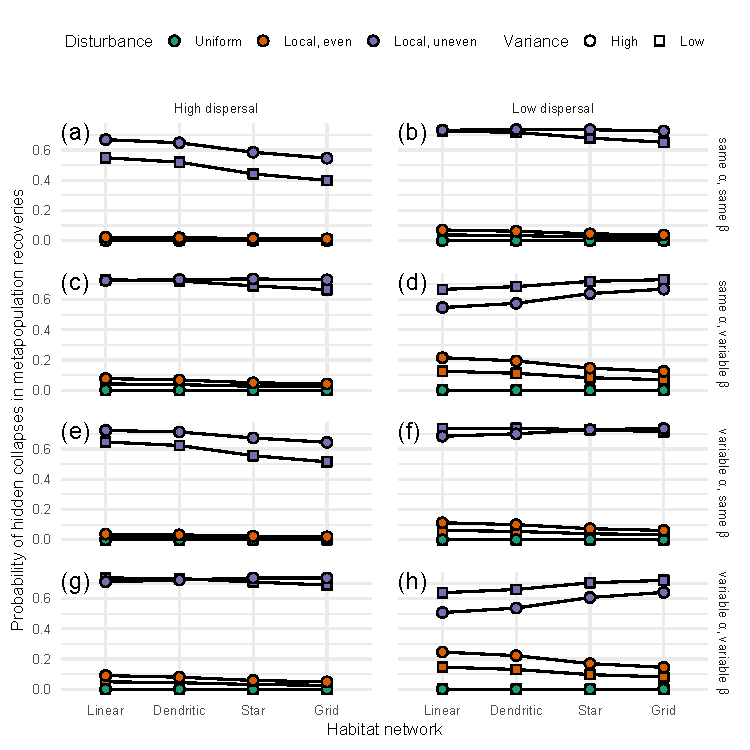
\includegraphics{Managing_for_ecological_surprises_in_metapopulations_files/figure-latex/conditional probability for hidden collapses-1} 

}

\caption{The probability of hidden local collapses in metapopulation recoveries depended on the interplay between network structure, dispersal (low≤0.001; high>0.001), spatial disturbances, heterogeneity in local demographic rates ($\alpha$ is local patch productivity and $\beta$ is local patch carrying capacity), and spatial-temporal recruitment variation (high=$\rho$=0.6 and $\sigma$=0.1; low=$\rho$≈0 and $\sigma$= 0.001).}\label{fig:conditional probability for hidden collapses}
\end{figure}

\begin{figure}[H]

{\centering 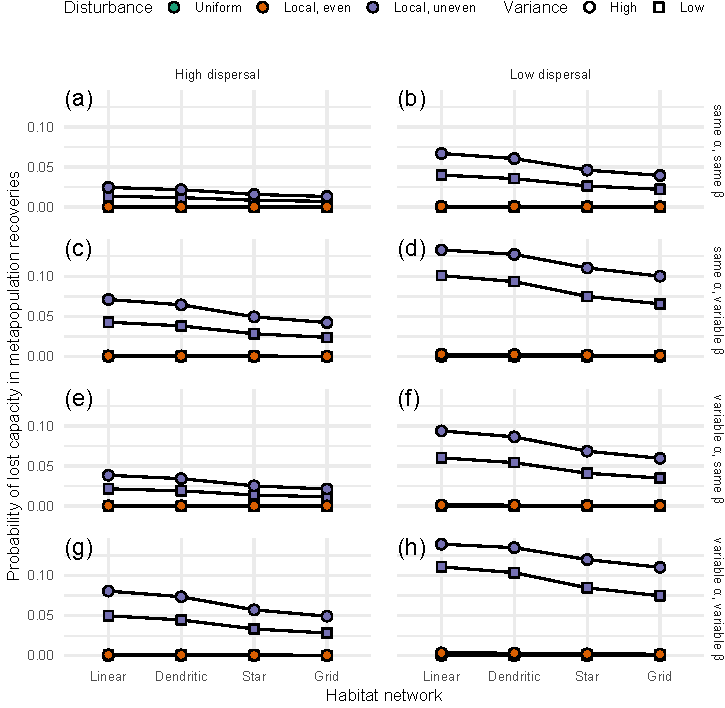
\includegraphics{Managing_for_ecological_surprises_in_metapopulations_files/figure-latex/conditional probability for lost capacity-1} 

}

\caption{The probability of lost productive capacity in metapopulation recoveries depended on the interplay between network structure, dispersal (low≤0.001; high>0.001), spatial disturbances, heterogeneity in local demographic rates ($\alpha$ is local patch productivity and $\beta$ is local patch carrying capacity), and spatial-temporal recruitment variation (high=$\rho$=0.6 and $\sigma$=0.1; low=$\rho$≈0 and $\sigma$= 0.001).}\label{fig:conditional probability for lost capacity}
\end{figure}

\hypertarget{references}{%
\subsection{References}\label{references}}

\vspace{3truemm}

\hypertarget{refs}{}
\begin{CSLReferences}{1}{0}
\leavevmode\vadjust pre{\hypertarget{ref-Anderson2015}{}}%
Anderson, S.C., Moore, J.W., McClure, M.M., Dulvy, N.K. \& Cooper, A.B.
(2015). {Portfolio conservation of metapopulations under climate
change.} \emph{Ecological Applications}, 25, 559--572.

\leavevmode\vadjust pre{\hypertarget{ref-Bowlby2020}{}}%
Bowlby, H.D. \& Gibson, A.J.F. (2020).
\href{https://doi.org/10.1139/cjfas-2019-0001}{{Evaluating whether
metapopulation structure benefits endangered diadromous fishes}}.
\emph{Canadian Journal of Fisheries and Aquatic Sciences}, 77, 388--400.

\leavevmode\vadjust pre{\hypertarget{ref-Csardi2006}{}}%
Csardi, G. \& Nepusz, T. (2006). \href{https://igraph.org}{{The igraph
software package for complex network research}}. \emph{InterJournal},
Complex Sy, 1695.

\leavevmode\vadjust pre{\hypertarget{ref-Forrest2010}{}}%
Forrest, R.E., McAllister, M.K., Dorn, M.W., Martell, S.J.D. \& Stanley,
R.D. (2010). \href{https://doi.org/10.1139/f10-077}{{Hierarchical
Bayesian estimation of recruitment parameters and reference points for
Pacific rockfishes (Sebastes spp.) under alternative assumptions about
the stock--recruit function}}. \emph{Canadian Journal of Fisheries and
Aquatic Sciences}, 67, 1611--1634.

\leavevmode\vadjust pre{\hypertarget{ref-Fullerton2016}{}}%
Fullerton, A.H., Anzalone, S., Moran, P., Van Doornik, D.M., Copeland,
T. \& Zabel, R.W. (2016).
\href{https://doi.org/10.1002/eap.1411}{{Setting spatial conservation
priorities despite incomplete data for characterizing metapopulations}}.
\emph{Ecological Applications}, 26, 2558--2578.

\leavevmode\vadjust pre{\hypertarget{ref-Hennig2014}{}}%
Hennig, C. (2014). {How many bee species? A case study in determining
the number of clusters}. In: \emph{Data analysis, machine learning and
knowledge discovery} (eds. Spiliopoulou, M., Schmidt-Thieme, L. \&
Janning, R.). pp. 41--49.

\leavevmode\vadjust pre{\hypertarget{ref-Moore2021}{}}%
Moore, J.W., Connors, B.M. \& Hodgson, E.E. (2021).
\href{https://doi.org/10.1111/faf.12567}{{Conservation risks and
portfolio effects in mixed‐stock fisheries}}. \emph{Fish and Fisheries},
faf.12567.

\leavevmode\vadjust pre{\hypertarget{ref-Murtagh2014}{}}%
Murtagh, F. \& Legendre, P. (2014).
\href{https://doi.org/10.1007/s00357-014-9161-z}{{Ward's hierarchical
agglomerative clustering method: which algorithms implement Ward's
criterion?}} \emph{Journal of Classification}, 31, 274--295.

\leavevmode\vadjust pre{\hypertarget{ref-Myers1999}{}}%
Myers, R.A., Bowen, K.G. \& Barrowman, N.J. (1999).
\href{https://doi.org/10.1139/f99-201}{{Maximum reproductive rate of
fish at low population sizes}}. \emph{Canadian Journal of Fisheries and
Aquatic Sciences}, 56, 2404--2419.

\leavevmode\vadjust pre{\hypertarget{ref-Okamoto2020}{}}%
Okamoto, D.K., Hessing‐Lewis, M., Samhouri, J.F., Shelton, A.O., Stier,
A.C., Levin, P.S. \& Salomon, A.K. (2020).
\href{https://doi.org/10.1002/eap.2051}{{Spatial variation in exploited
metapopulations obscures risk of collapse}}. \emph{Ecological
Applications}, 30, e02051.

\leavevmode\vadjust pre{\hypertarget{ref-Walters2004}{}}%
Walters, C.J. \& Martell, S.J.D. (2004). \emph{{Fisheries ecology and
management}}. Princeton University Press.

\leavevmode\vadjust pre{\hypertarget{ref-Yeakel2014}{}}%
Yeakel, J.D., Moore, J.W., Guimarães, P.R. \& Aguiar, M.A.M. de. (2014).
\href{https://doi.org/10.1111/ele.12228}{{Synchronisation and stability
in river metapopulation networks}}. \emph{Ecology Letters}, 17,
273--283.

\leavevmode\vadjust pre{\hypertarget{ref-Zelnik2019}{}}%
Zelnik, Y.R., Arnoldi, J. \& Loreau, M. (2019).
\href{https://doi.org/10.1002/ecy.2446}{{The three regimes of spatial
recovery}}. \emph{Ecology}, 100, e02586.

\end{CSLReferences}

\end{document}
